\section{Codificação das instruções}
  Nesta arquitetura temos 64 instruções distribuídas da seguinte forma: 40 instruções de operações aritméticas, lógicas, multiplicação/divisão e de deslocamento, 6 de testes condicionais e operações condicionais de troca, 4 de operações de acesso ao acumulador, 8 de saltos e \textit{branches} e por fim mais 6 de operações de \textit{load} e \textit{store}. Todas as instruções contém 32 bits. Exitem três formatos de instruções: \textit{R} (\textit{R-type}), \textit{I} (\textit{I-type}) e \textit{Jump}. Ainda nesta sessão os OPCODES de cada instrução serão apresentados de forma binaria.
  
  \FloatBarrier
    \begin{center}
\begin{longtable}[pos]{|m{2cm} | m{1cm} | m{8cm}|} \hline    
          \multicolumn{1}{|c|}{\cellcolor[gray]{0.9}\textbf{Formato da instrução}} & 
          \multicolumn{1}{c|}{\cellcolor[gray]{0.9}\textbf{Instrução}} & 
          \multicolumn{1}{l|}{\cellcolor[gray]{0.9}\textbf{Descrição}} \\ \hline
          \endfirsthead
          \hline
          \multicolumn{3}{|l|}
          {{\bfseries continuação da página anterior}} \\
          \hline
          \multicolumn{1}{|c|}{\cellcolor[gray]{0.9}\textbf{Formato da Instrução}} & 
          \multicolumn{1}{c|}{\cellcolor[gray]{0.9}\textbf{Instrução}} & 
          \multicolumn{1}{l|}{\cellcolor[gray]{0.9}\textbf{Descrição}} \\ \hline
          \endhead
            \hline
          \multicolumn{3}{|r|}{{\bfseries continua na próxima página}} \\ \hline
          \endfoot

          \hline
          \endlastfoot 
           
			\multirow{30}{*}{R-type} & ADD & Soma dois valores \\ \cline{2-3}
			& ADDU & Soma dois valores sem sinal \\ \cline{2-3}
			& CLO & Conta quantos 1's existem no registrador $RS$ da esquerda para a direita até o primeiro 0 \\ \cline{2-3}
			& CLZ &  Conta quantos 0's existem em $RS$ da esquerda para a direita até o primeiro 1\\ \cline{2-3}
			& SUB & Subtrai dois valores  \\ \cline{2-3}
			& SUBU & Subtrai dois valores sem sinal \\ \cline{2-3}
			& SEB & Estende o dado em 1 byte \\ \cline{2-3}
			& SEH & Estende o dado em metade de uma palavra, ou seja,  2 bytes \\ \cline{2-3}
			& SLL & Desloca a palavra para a esquerda em 5 bits \\ \cline{2-3}
			& SLLV & Desloca $RS$ para a esquerda pelo valor dos 5 bits menos significativos de$RT$ \\ \cline{2-3}
			& SRA & Desloca a palavra para a direita em 5 bits sinalizados \\ \cline{2-3}
			& SRAV & Desloca $RS$ para a direita pelo valor dos 5 bits menos significativos de $RT$ \\ \cline{2-3}
			& SRL &  Desloca a palavra para a direita em 5 bits \\ \cline{2-3}
			& SRLV & Desloca $RS$ para a direita pelo valor dos 5 bits, sem sinal, menos significativos de $RT$  \\ \cline{2-3}
			& AND & AND lógico de dois valores \\ \cline{2-3}
			& NOR & OR lógico de dois valores negado \\ \cline{2-3}
			& OR &  OR lógico de dois valores\\ \cline{2-3}
			& XOR & OR lógico exclusivo de dois valores \\ \cline{2-3}
			& DIV &  Divisão de dois valores onde o resto fica no registrador $HI$ e o quociente no $LO$\\ \cline{2-3}
			& DIVU &  Divisão de dois valores sem sinal onde o resto fica no registrador $HI$ e o quociente no $LO$  \\ \cline{2-3}
			& MADD &  Multiplica dois valores e soma a outro valor anterior\\ \cline{2-3}
			& MADDU & Multiplica dois valores sem sinal e soma a outro valor anterior \\ \cline{2-3}
			& MSUB &  Multiplica dois valores e subtrai a outro valor anterior\\ \cline{2-3}
			& MSUBU & Multiplica dois valores sem sinal e subtrai a outro valor anterior \\ \cline{2-3}
			& MUL & Multiplica dois valores  \\ \cline{2-3}
			& MULT & Multiplica dois valores de 32 bits e salva em dois registradores $HI$ e $LO$ \\ \cline{2-3}
			& MULTU & Multiplica dois valores sem sinal de 32 bits e salva em dois registradores $HI$ e $LO$ \\ \cline{2-3}
			& MFHI & Move um dado de $RD$ para $HI$ \\ \cline{2-3}
			& MFLO & Move um dado de $RD$ para $LO$ \\ \cline{2-3}
			& MTHI & Move um dado de $HI$ para $RS$ \\ \cline{2-3}
			& MTLO & Move um dado de $LO$ para $RS$ \\ \cline{2-3}
			& JR & Pula para o endereço que está em $RS$ \\ \cline{2-3}
			& JALR & Guarda o valor atual de PC mais 4 em $RD$ e pula para o endereço que está em $RS$ \\ \cline{2-3}
			& MOVN & Move o que está em $RS$ para $RD$ se o dado de $RT$ for diferente de 0  \\ \cline{2-3}
			& MOVZ & Move o que está em $RS$ para $RD$ se o dado de $RT$ for igual a 0  \\ \cline{2-3}
			& SLT & Guarda em $RD$ 1, se o dado de $RS$ for menor que o de $RT$, senão guarda 0 \\ \cline{2-3}
			& SLTU & Guarda em $RD$ 1, se o dado de $RS$ for menor que o de $RT$, sendo ambos sem sinal, senão guarda 0 \\ \cline{2-3}
			& WSBH &  \\ \cline{2-3}
			& MOVE & Atribui o valor do registrador $RS$ ao $RD$ \\\hline
			& NOP & Não realiza nenhuma operação \\\hline
	\multirow{20}{*}{I-type} & ADDI & Soma dois valores, um destes imediato \\ \cline{2-3}
	& ADDIU & Soma dois valores, um destes imeditao, ambos sem sinal \\ \cline{2-3}
	& LUI & Desloca para a direita o imediato, em 16 bits \\ \cline{2-3}
	& ANDI & AND lógico de dois valores, um destes imediato \\ \cline{2-3}
	& ORI & OR lógico de dois valores, um destes imediato \\ \cline{2-3}
	& XORI & OR exclusivo de dois valores, um destes imediato \\ \cline{2-3}
	& BGEZ & Altera o valor de PC para o PC atual mais o imediato de 18 bits, se o dado em $RS$ for maior igual a 0 \\ \cline{2-3}
	& BLTZ & Altera o valor de PC para o PC atual mais o imediato de 18 bits, se o dado em $RS$ for menor que 0 \\ \cline{2-3}
	& BEQ & Altera o valor de PC para o PC atual mais o imediato de 18 bits, se o dado em $RS$ for igual ao de $RT$ \\ \cline{2-3}
	& BNE &  Altera o valor de PC para o PC atual mais o imediato de 18 bits, se o dado em $RS$ for diferente ao de $RT$\\ \cline{2-3}
	& LB & Busca na posição $RS+Offset16$ e guarda em $RT$ o byte \\ \cline{2-3}
	& LW & Busca na posição $RS+Offset16$ e guarda em $RT$ a palavra \\ \cline{2-3}
	& SB & Guarda o byte que está em $RT$, na posição $RS+Offset16$ da memória \\ \cline{2-3}
	& SW & Guarda a palavra que está em $RT$, na posição $RS+Offset16$ da memória \\ \cline{2-3}
	& LH & Busca na posição $RS+Offset16$ e guarda em $RT$ um dado de 16 bits\\ \cline{2-3}
	& SH & Guarda um dado de 16 bits que está em $RT$, na posição $RS+Offset16$ da memória \\ \cline{2-3}
	& SLTI & Guarda em $RD$ 1, se o dado de $RS$ for menor que o valor imediato, senão guarda 0 \\ \cline{2-3}
	& SLTIU & Guarda em $RD$ 1, se o dado de $RS$ sem sinal for menor que o valor imediato, senão guarda 0 \\ \cline{2-3}
	& LA & Carrega o valor de uma label como imediato \\ \cline{2-3}
	& LI & Carrega uma constantede 32 bits ao registrador $RD$ \\\hline
	\multirow{2}{*}{Jump} & J & Altera o PC para o endereço vindo na instrução \\ \cline{2-3}
	& JAL & Guarda o PC mais 4 em \textit{RA} e altera o PC para o endereço vindo na instrução \\\hline
\end{longtable}
\end{center}

	O formato \textit{R} está relacionado as instruções lógicas, aritméticas, deslocamento, acesso ao acumulador e operações condicionais.
	\begin{figure}[H]
    	\centering
    	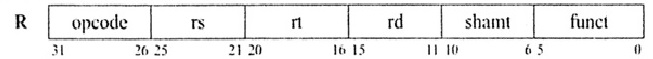
\includegraphics{R-type}
	\end{figure}
	
\begin{table}[H]
\centering	
\begin{tabular}{|c|l|}
	\hline 
	\cellcolor[gray]{0.9}\textbf{CAMPO} & \cellcolor[gray]{0.9}\textbf{DESCRIÇÃO} \\ 
	\hline 
	\textit{OPCODE} & Código da operação básica da instrução. \\ 
	\hline 
	\textit{RS} & Registrador do primeiro operando de origem. \\ 
	\hline 
	\textit{RT} & Registrador do segundo operando de origem. \\ 
	\hline 
	\textit{RD} & Registrador de destino. \\ 
	\hline 
	\textit{SHAMT} & Quantidade de deslocamento. \\ 
	\hline 
	\textit{FUNCT} & Variante específica da operação. \\ 
	\hline 
	\end{tabular} 
	\end{table}
	
	Um segundo tipo de formato de instrução é chamado de formato \textit{I}, utilizado pelas instruções imediatas, lógicas.
	\begin{figure}[H]
    	\centering
    	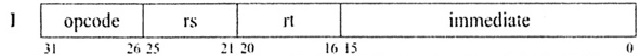
\includegraphics{I-Type}
  	\end{figure}
  	
  	\begin{table}[H]
\centering	
\begin{tabular}{|c|l|}
	\hline 
	\cellcolor[gray]{0.9}\textbf{CAMPO} & \cellcolor[gray]{0.9}\textbf{DESCRIÇÃO} \\ 
	\hline 
	\textit{OPCODE} & Código da operação básica da instrução. \\ 
	\hline 
	\textit{RS} & Registrador do primeiro operando de origem. \\ 
	\hline 
	\textit{RT} & Registrador de destino. \\ 
	\hline 
	\textit{IMMEDIATE} & Constante numérica. \\ 
	\hline 
	\end{tabular} 
	\end{table}
	
	O formato \textit{Jump} serve para as instruções de desvio condicional e incondicional. 
 	
   	\begin{figure}[H]
    	\centering
    	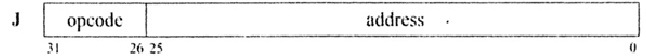
\includegraphics{J-Type}
		\label{jump}
  	\end{figure}
  	
  	\begin{table}[H]
\centering	
\begin{tabular}{|c|l|}
	\hline 
	\cellcolor[gray]{0.9}\textbf{CAMPO} & \cellcolor[gray]{0.9}\textbf{DESCRIÇÃO} \\ 
	\hline 
	\textit{OPCODE} & Código da operação básica da instrução. \\ 
	\hline 
	\textit{ADDRESS} & Endereço de memória. \\ 
	\hline 
	\end{tabular} 
	\end{table}

Instruções Aritméticas
\begin{table}[H]
\centering
	\begin{tabular}{|c|c|c|}
  	\hline 
  	\cellcolor[gray]{0.9}\textbf{OPCODE} & \cellcolor[gray]{0.9}\textbf{INSTRUCTION} & \cellcolor[gray]{0.9}\textbf{FUNCTION} \\ 
  	\hline 
  	000000 & ADD & 100000 \\ 
  	\hline 
  	001000 & ADDI & -\\ 
  	\hline 
  	001001 & ADDIU & - \\ 
  	\hline 
  	000000 & ADDU & 100001 \\ 
  	\hline 
  	000000 & CLO & 010001 \\ 
  	\hline 
  	000000 & CLZ & 100000 \\ 
  	\hline  
  	000000 & SUB & 100010 \\ 
  	\hline
  	000000 & SUBU & 100011 \\
  	\hline 
  	011111 & SEB & 100000 \\
  	\hline 
  	011111 & SEH & 100000 \\
  	\hline 
  	001111 & LUI & - \\
  	\hline 
  	001001 & LA & - \\
  	\hline
  	001101 & LI & - \\
  	\hline
  	000000 & MOVE & 100000 \\
  	\hline
  	
  	\end{tabular} 
  \end{table} 
  	 	
Operações de Multiplicação e Divisão
\begin{table}[H]
\centering
	\begin{tabular}{|c|c|c|}
  	\hline 
  	\cellcolor[gray]{0.9}\textbf{OPCODE} & \cellcolor[gray]{0.9}\textbf{INSTRUCTION} & \cellcolor[gray]{0.9}\textbf{FUNCTION} \\ 
  	\hline 
  	000000 & DIV & 011010 \\ 
  	\hline 
  	000000 & DIVU & 011011 \\ 
  	\hline 
  	011100 & MADD & 000000 \\ 
  	\hline 
  	011100 & MADDU & 000001 \\ 
  	\hline  
  	011100 & MSUB & 000100 \\ 
  	\hline
  	011100 & MSUBU & 000101 \\
  	\hline 
  	011100 & MUL & 000010 \\
  	\hline 
  	000000 & MULT & 011000 \\
  	\hline
  	000000 & MULTU & 011001 \\
  	\hline
  	\end{tabular} 
  \end{table} 
	
Instruções Lógicas
\begin{table}[H]
\centering	
\begin{tabular}{|c|c|c|}
	\hline 
  \cellcolor[gray]{0.9}\textbf{OPCODE} & \cellcolor[gray]{0.9}\textbf{INSTRUCTION} & \cellcolor[gray]{0.9}\textbf{FUNCTION} \\ 
  	\hline 
	000000 & AND & 100100 \\ 
	\hline 
	001100 & ANDI & -\\ 
	\hline 
	000000 & NOR & 100111\\ 
	\hline 
	000000 & OR & 100101\\ 
	\hline
	001101 & ORI & -\\ 
	\hline 
	000000 & XOR & 100110 \\
	\hline
	001110 & XORI & -\\ 
  	\hline 
  	000000 & NOP & 000000\\ 
  	\hline
	\end{tabular} 
\end{table}	
	
Instruções de Acesso ao Acumulador
\begin{table}[H]
\centering 	
  	\begin{tabular}{|c|c|c|}
  	\hline 
  	\cellcolor[gray]{0.9}\textbf{OPCODE} & \cellcolor[gray]{0.9}\textbf{INSTRUCTION} & \cellcolor[gray]{0.9}\textbf{FUNCTION} \\ 
  	\hline 
  	000000 & MFHI & 010000 \\ 
  	\hline 
  	000000 & MFLO & 010010 \\ 
  	\hline 
  	000000 & MTHI & 010001 \\ 
  	\hline 
  	000000 & MTLO & 010011 \\ 
  	\hline 
  	\end{tabular} 
\end{table}

Instruções de Deslocamento
\begin{table}[H]
\centering 	
  	\begin{tabular}{|c|c|c|}
  	\hline 
  	\cellcolor[gray]{0.9}\textbf{OPCODE} & \cellcolor[gray]{0.9}\textbf{INSTRUCTION} & \cellcolor[gray]{0.9}\textbf{FUNCTION} \\ 
  	\hline 
  	000000 & SLL & 000000\\ 
  	\hline 
  	000000 & SLLV & 000100\\ 
  	\hline 
  	000000 & SRA & 000011 \\ 
  	\hline 
  	000000 & SRAV & 000111 \\ 
  	\hline
  	000000 & SRL & 000010 \\ 
  	\hline 
  	000000 & SRLV & 000110 \\ 
  	\hline 
  	\end{tabular} 
\end{table}

Instruções Condicionais
\begin{table}[H]
\centering 	
  	\begin{tabular}{|c|c|c|}
  	\hline 
  \cellcolor[gray]{0.9}\textbf{OPCODE} & \cellcolor[gray]{0.9}\textbf{INSTRUCTION} & \cellcolor[gray]{0.9}\textbf{FUNCTION} \\ 
  	\hline  
  	000000 & MOVN & 001011 \\ 
  	\hline 
  	000000 & MOVZ & 001010 \\ 
  	\hline 
  	000000 & SLT & 101010 \\ 
  	\hline 
  	001010 & SLTI & -\\ 
  	\hline 
  	001011 & SLTIU & -\\ 
  	\hline 
  	000000 & SLTU & 101011 \\ 
  	\hline 
  	\end{tabular} 
\end{table}

Instruções de Jump e Branch
\begin{table}[H]
\centering 	
  	\begin{tabular}{|c|c|c|}
  	\hline 
  	 \cellcolor[gray]{0.9}\textbf{OPCODE} & \cellcolor[gray]{0.9}\textbf{INSTRUCTION} & \cellcolor[gray]{0.9}\textbf{FUNCTION} \\ 
  	\hline  
  	000001 & BQEZ &-\\ 
  	\hline 
  	000001 & BLTZ &-\\ 
  	\hline 
  	000100 & BEQ &-\\ 
  	\hline 
  	000101 & BNE &-\\ 
  	\hline 
  	000010 & J &-\\ 
  	\hline 
  	000000 & JR & 001000 \\ 
  	\hline
  	000011 & JAL &-\\ 
  	\hline
  	000000 & JALR & 001001 \\ 
  	\hline
  	
  	\end{tabular} 
\end{table}

Instruções de Load e Store
\begin{table}[H]
\centering 	
  	\begin{tabular}{|c|c|}
  	\hline 
  	\cellcolor[gray]{0.9}\textbf{OPCODE} & \cellcolor[gray]{0.9}\textbf{INSTRUCTION} \\ 
  	\hline 
  	100000 & LB \\ 
  	\hline 
  	100011 & LW \\ 
  	\hline 
  	101000 & SB \\ 
  	\hline 
  	101011 & SW \\ 
  	\hline 
  	100001 & LH \\ 
  	\hline
  	101001 & SH \\ 
  	\hline 
  	\end{tabular} 
\end{table}